\chapter{Real-Time Implementation and Control}\label{ch:realtime}

\begin{flushright}{\it
    ``The real problem is that programmers have spent far too much time worrying \\
    about efficiency in the wrong places and at the wrong times; premature\\
    optimization is the root of all evil (or at least most of it) in programming.''\\
    - Donald E. Knuth}
\end{flushright}
%
\vspace{2em}
\todo{check if all references to this chapter are actually touched upon in here}
\noindent A large part of this PhD project has been to implement novel combinations of existing FD schemes in real time (see Section \ref{sec:objectivesContributions}). As opposed to many FDTD-based musical instruments found in the literature, those presented in this work, allow for real-time control such the virtual instrument can be played. 

Many simulations are focused on accuracy and

Real-time implementations of FD schemes 

physical models
Give overall structure of code

Important to find the balance between accuracy and sound. 

Implementation of the physical models
using FDTD methods

As mentioned in Chapter \ref{ch:physMod}, FDTD methods are used for high-quality and accurate simulations, rather than for real-time applications. This is due to their lack of simplifications.

Usually, \texttt{MATLAB} is used for simulating 

Here, an interactive application is considered real-time when
\begin{center}\it
    Control of the application generates or manipulates audio with no noticeable latency.
\end{center}

For human-computer interaction, the task at hand greatly determines how much latency is acceptable. Wessel and Wright \cite{Wessel2002} place the upper limit of latency when interacting with computers for musical purposes at $10$ ms. Moreover, they place the a limit on the \textit{jitter}, or of variation of the latency, at $1$ ms. It is thus important to keep the CPU usage at a fixed level as much as possible, and different ways of controlling and interacting with the application should not influence the number of computations much.

Also the application needs to be controlled continuously

As a large contribution of this PhD project was the real-time implementation of the physical models presented in 

Finite representation: $1.80\cdot 10^{308}$


Apart from being able to be used by musicians, real-time implementations can truly help to (informally) evaluate the models by interacting with it in a natural way (rather than static parameters).


\todo{Figure with programming languages sorted by speed}




Although \texttt{MATLAB} is a great tool for prototyping, it is a \textit{high-level} programming language, i.e., has a high level of abstraction. Generally, higher-level programming languages are easier to program, but more control -- and speed -- is gained by using a lower-level programming language such as C++.

It must be said that \texttt{MATLAB} is highly optimised for large matrix computations.

A great framework for real-time audio programming is provided by JUCE.\footnote{\url{https://juce.com/}} This framework provides functionality that handles the backend of  an application and specifically allows for audio and graphics to run simultaneously on separate threads. All real-time instrument simulations made over the course of this PhD project have been implemented using the JUCE framework. 


some details on this will be given. 
This chapter provides information on the real-time implementations made during this PhD project

This chapter can be considered a general contribution that can be applied to all papers in Part \ref{part:papers} (except paper \citeP[G]). The most important aspects of the implementation will be highlighted.

Firstly, details on the structure of a class implementing a FD scheme will be provided, using the damped stiff string as an example. Secondly, an overall code structure is given that can be applied to many applications created during this PhD project.   

Then... 

Finally, this chapter will present the Sensel Morph and the PHANTOM Omni, two hardware devices which have been used to control the physical models presented in papers \citeP[A], \citeP[B], \citeP[C], \citeP[D] and \citeP[E].

\section{Real-time FD schemes}\label{sec:realTimeFDScheme}
Until now, this thesis presented matrix form of schemes (see e.g. Eqs. \eqref{eq:matrixFormStiffString} and \eqref{eq:matrixFormThinPlate}) for a compact implementation in \texttt{MATLAB}. Although libraries for handling matrices in C++ exist, the highest algorithm speed is obtained by using the update equations directly.

In any of the real-time applications created during this project, the update equation implementing an FD scheme is always most computationally expensive part. This algorithm needs to run 44100x per second, whereas the rest of the implementation can run at a much lower rate. This section provides details and considerations on the real-time implementation of FD schemes in C++ during this project. The damped stiff string presented in Chapter \ref{ch:stiffString} will be used an example. The full implementation can be found online and parts will be presented here to aid the explanation.\footnote{\url{https://github.com/SilvinWillemsen/SimpleStringApp/}} The FD scheme is implemented in a separate class called \texttt{SimpleString}, and will be used in the following explanation.

% Before going into the implementation of the update equation, this section provides the setup necessary for the implementation.

\subsection{System states and pointer switches}\label{sec:pointerSwitch}
In any FD scheme implementation, at the end of every iteration, the system states must be updated, i.e., the following operations must be performed:
\begin{equation*}
    \u^{n-1} := \u^{n} \qaq \u^{n} := \u^{n+1}.
\end{equation*}
In \texttt{MATLAB}, one would simply perform these operations according to

\setlstMAT
\begin{lstlisting}[belowskip=-0.5\baselineskip]
for n = 1:lengthSound
    ...
    uPrev = u;
    u = uNext;
end
\end{lstlisting}
In C++, however, one has the ability to perform a \textit{pointer switch} to update the system states. For a 1D FD scheme with $N+1$ grid points, the number of copy-operations it takes to update the system states manually would be $2(N+1)$, as shown in Figure \ref{fig:vectorCopy}. A pointer switch, as shown in Figure \ref{fig:pointerSwitch}, only needs 4 copy-operations per iteration and can be carried out in C++ as follows:

\setlstCpp
\begin{lstlisting}[belowskip=-0.5\baselineskip]
double SimpleString::updateStates()
{
    double* uTmp = u[2];
    u[2] = u[1];
    u[1] = u[0];
    u[0] = uTmp;
}
\end{lstlisting}
Here, \texttt{u} is a vector containing 3 pointers, each of which points a state vector at a certain time step: 
\begin{equation}
    \texttt{u[0]} \rightarrow \u^{n+1}, \quad \texttt{u[1]} \rightarrow \u^{n}, \qaq \texttt{u[2]} \rightarrow \u^{n-1}.
\end{equation}
A temporary pointer is assigned to where the $\u^{n-1}$ pointer is currently pointing at, to be able to assign that location in memory to the $\u^{n+1}$ pointer in the end. The values of that vector will be overwritten by the update equation in the next iteration (see Section \ref{sec:updateEquationCpp} and Figure \ref{fig:pointerSwitchFull}).

\begin{figure}[t]
    \centering
    \subfloat[Copying values: $2(N+1)$ operations per iteration. \label{fig:vectorCopy}]{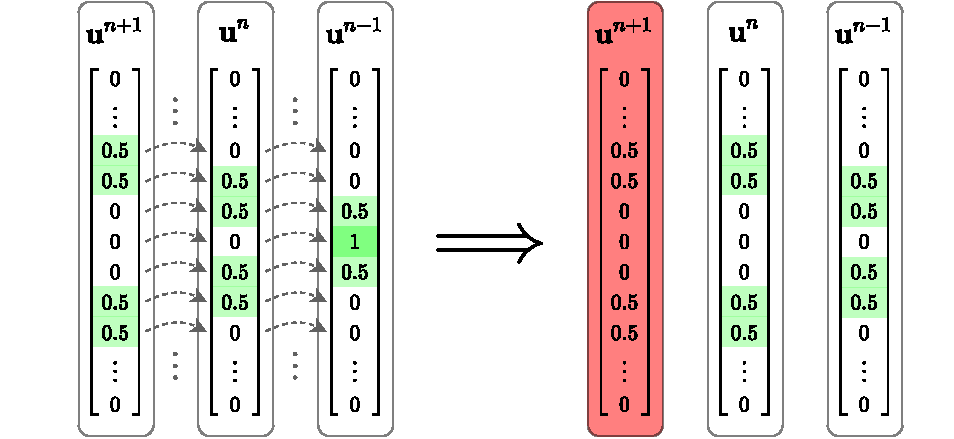
\includegraphics[width=0.8\textwidth]{figures/realtime/vectorCopy.pdf}}\\
    \subfloat[Pointer switch: 4 operations per iteration. \label{fig:pointerSwitch}]{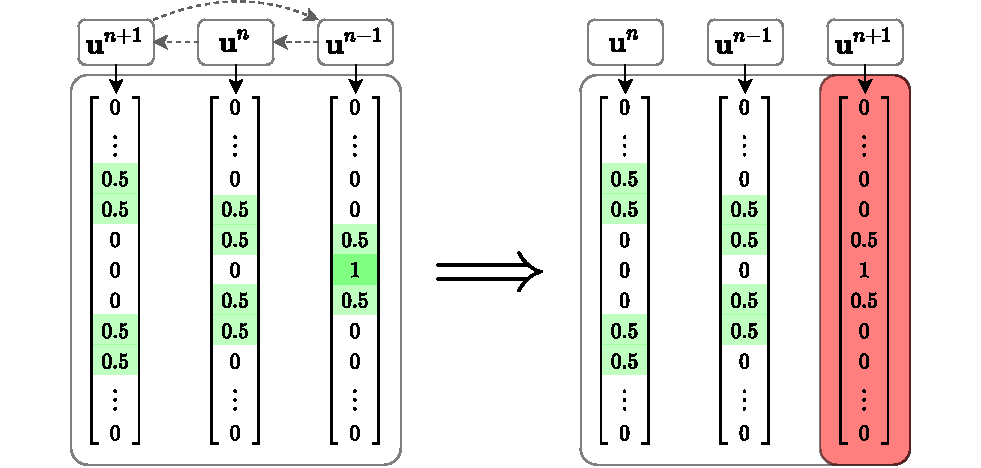
\includegraphics[width=0.8\textwidth]{figures/realtime/pointerSwitch.pdf}}
    \caption{Updating the state vectors by (a) copying all values individually, or (b) performing a pointer switch. Non-zero values are highlighted in green for clarity. The values of the red vector will be overwritten by the update of the scheme in the next iteration so these values will no longer be used.\label{fig:pointerSwitchFull}}
\end{figure}

The state vectors themselves are stored in a matrix (which is a `vector of vectors' in C++). This matrix will have 3 columns related to the 3 time steps required in the FD scheme, and $N+1$ rows, which is the number of grid points.\footnote{These are not actual rows and columns as in a matrix, but are used here for ease of explanation.} The matrix is initialised as follows

\setlstCpp
\begin{lstlisting}[belowskip=-0.5\baselineskip]
//// In the constructor of SimpleString////

// initialise vectors
uStates = std::vector<std::vector<double>> (3, 
                                    std::vector<double>(N+1, 0));
\end{lstlisting}
%
Next, the aforementioned pointers are initialised such that they contain the to the memory addresses of the first indices of the three state vectors in the matrix.

\begin{lstlisting}[belowskip=-0.5\baselineskip]
//// In the constructor of SimpleString ////

// Initialise pointer vector
u.resize (3, nullptr);

// Make set memory addresses to first index of the state vectors.
for (int i = 0; i < 3; ++i)
    u[i] = &uStates[i][0];
\end{lstlisting}
One will then be able to work with the pointers directly in the eventual update equation (see Section \ref{sec:updateEquationCpp}).

\subsection{Precalculation}
To prevent extra computations in the FD scheme, one wants to calculate as many of the coefficients possible beforehand, as these (generally) do not vary over time. Recalling the update equation for a stiff string in Eq. \eqref{eq:stiffStringUpdate}, one can write this as
\begin{equation}
    \begin{aligned}
        A_\text{div} u_l^{n+1} &= B_1 \uln + B_2 (u_{l+1}^n + u_{l-1}^n) + B_3(u_{l+2}^n + u_{l-2}^n) \\
        &\quad+ C_1u_l^{n-1}+ C_2(u_{l+1}^{n-1} + u_{l-1}^{n-1}),
    \end{aligned}
    \end{equation}
where
\begin{gather*}
    A_\text{div} = 1+\sz k, \quad B_0 = 2 - 2\lambda^2 - 6\mu^2 - \frac{4\so k}{h^2}, \quad B_1 = \lambda^2 + 4\mu^2 + \frac{2\so k}{h^2},\\
    B_2 = - \mu^2, \quad C_0 = -1+\sz k + \frac{4\so k}{h^2},\qaq C_1 = - \frac{2\so k}{h^2}.
\end{gather*}
All these coefficients can be calculated in the constructor of the stiff string class. One can also already divide the $B$ and $C$ coefficients by $A_\text{div}$ as done in the code below.
\setlstCpp
\begin{lstlisting}[]
//// In the constructor of SimpleString ////

// Coefficients used for damping
S0 = sigma0 * k;
S1 = (2.0 * sigma1 * k) / (h * h);

// Scheme coefficients
B0 = 2.0 - 2.0 * lambdaSq - 6.0 * muSq - 2.0 * S1; // u_l^n
B1 = lambdaSq + 4.0 * muSq + S1;                   // u_{l+-1}^n
B2 = -muSq;                                        // u_{l+-2}^n
C0 = -1.0 + S1 + 2.0 * S2;                         // u_l^{n-1}
C1 = -S1;                                          // u_{l+-1}^{n-1}

Adiv = 1.0 / (1.0 + S0);                           // u_l^{n+1}

// Divide by u_l^{n+1} term
B0 *= Adiv;
B1 *= Adiv;
B2 *= Adiv;
C0 *= Adiv;
C1 *= Adiv;
\end{lstlisting}

\subsection{Update equation}\label{sec:updateEquationCpp}
With all the above set up, the update equation can be implemented as follows:

\begin{lstlisting}[belowskip=-0.5\baselineskip]
void SimpleString::calculateScheme()
{
    for (int l = 2; l < N-1; ++l) // clamped boundaries
            u[0][l] = B1 * u[1][l] + B2 * (u[1][l + 1] + u[1][l - 1]) 
                + B3 * (u[1][l + 2] + u[1][l - 2])         
                + C1 * u[2][l] + C2 * (u[2][l + 1] + u[2][l - 1]);
}
\end{lstlisting}
This function and the pointer switch in Section \ref{sec:pointerSwitch} (in that order) will then have to be called once per sample.


\section{Code structure}\label{sec:codeStructure}
This section presents the general code structure used for the real-time applications created in this project. As an example, consider a simple instrument consisting of one string and one plate, and a connection between them as presented in Section \ref{sec:stringPlateConnection}. The string is excited using the Sensel Morph (see Section \ref{sec:sensel}). This is a simplified case of the contribution made in papers \citeP[A] and \citeP[B]. 

The structure of the code is visualised in Figure \ref{fig:codeStructure}. The white boxes denote various classes or components of the application which will be described in detail shortly. The black arrows indicate instructions, and hollow arrows indicate data flows. All arrows are accompanied by a box denoting the instruction / dataflow and the colour of the box denotes at what rate this happens.

\begin{figure}[h]
    \centering
    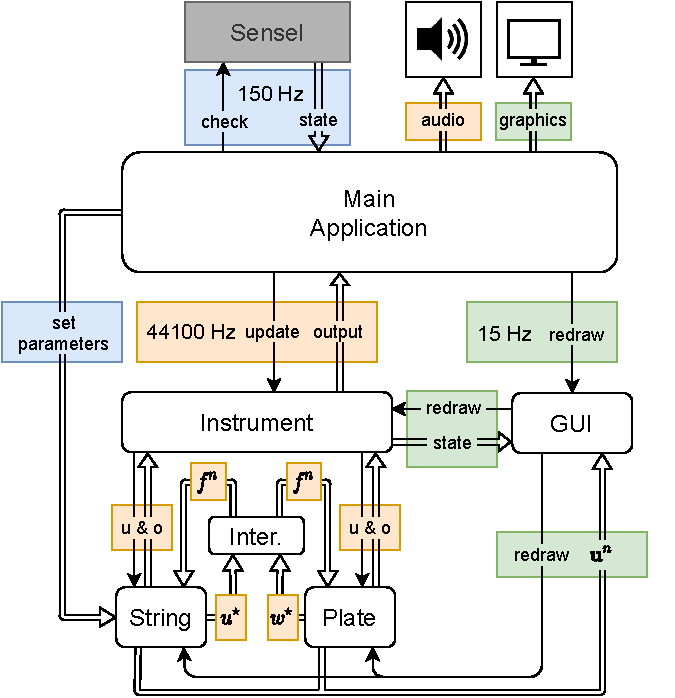
\includegraphics[width=0.8\textwidth]{figures/realtime/flowchart.pdf}
    \caption{The structure of a real-time implementation of a physical model. Boxes with `u \& o' refer to `update and output' and `Inter.' is short for `Interaction'. A detailed description of the figure is given in Section \ref{sec:codeStructure}. (Adapted from paper \citeP[A])\label{fig:codeStructure}}
\end{figure}

\subsubsection{Threads}
The application contains three different threads, all handled by the JUCE backend. The highest priority thread is the audio thread and is denoted by orange blocks. It runs at 44100 Hz and handles the calculations of the FD schemes. Denoted by blue, is the control thread and runs at 150 Hz. The input from the Sensel will be applied to the application at this rate. This rate corresponds to a maximum \textApprox 7 ms latency in control, which is below the upper limit for latency in musical applications proposed in \cite{Wessel2002}. Finally, the thread updating the graphical user interface (GUI) is set to run at 15 Hz, which is a value that was heuristically found to be a good balance between a smooth visuals and a fast application. %For powerful computers, or for low-complexity physical models, the speed could be increased. 
Papers \citeP[A], \citeP[C], and \citeP[H], contain a comparison between the speed of the application with and without the graphics. In all cases, results show that the graphics take up a large part of the computational power available.

\subsubsection{String and Plate}
The String and Plate classes implement the FD schemes of the stiff string and thin plate resonators respectively.\footnote{Note that the class can not actually be called `String' as this is already an existing variable type.} See Section \ref{sec:realTimeFDScheme} for an example of an implementation of the stiff string; a similar code structure can be used for the Plate class. As this section follows Section \ref{sec:stringPlateConnection}, the grid functions describing the string and the plate are defined as $\uqn$ and $\wlmn$, respectively. 

For the resonators to work in isolation, both classes require a function that calculates the scheme and one that updates their system states (see Section \ref{sec:realTimeFDScheme}). The interactions between the classes is handled by the Instrument class (see below). Therefore, both classes require additional functions that return $u^\star$ and $w^\star$ (see Figure \ref{fig:codeStructure}), as well as a function that adds the interaction force $f^n$ to the schemes. A final function on the audio  

Finally, the classes contain a `paint' function called by the GUI thread that visualises their state to the screen. 

\subsubsection{Instrument}
The Instrument class contains instances of the individual resonators and calls the functions that calculates the schemes and updates the states.

is called from the Main Application and contains instances of the individual resonators. Rather than performing the calculations of the FD schemes of these resonators, the Instrument class handles all interactions between the individual resonators. In the figure, this is denoted by the `Inter.' block and proceeds as follows:
\begin{enumerate}
    \item The instrument class retrieves the states of the schemes without the connection force. These are denoted by $u^\star$ and $w^\star$ and are calculated using in Eqs. \eqref{eq:stringPlateUStar} and \eqref{eq:stringPlateWStar}). These calculations are done in the String and Plate classes respectively (see below).
    \item The connection force $f^n$ is calculated using Eq. \eqref{eq:stringPlateForce}.
    \item The force is added to the scheme. 
\end{enumerate}

by the  the interaction between the string and the plate -- denoted by the `Inter.' block -- will be handled by the instrument class. It obtains the data needed to solve 

describes the interaction between the string and the plate and will be solved in the instrument class. 



The individual resonators could 


\subsubsection{Main Application}
The Main Application (also called MainComponent in JUCE) is the top-level class of the application that handles the audio input and output\footnote{This section assumes that the JUCE Audio Application template has been chosen -- not the Audio Plugin template.}

The main application contains an instance of the instrument class and calls a function 

Furthermore, it retrieves the output from the instrument which in turn retrieves it from the individual resonators.


Here, the interaction with the system is handled audio is handled.

Contains an instance of the instrument class


\subsection{Control}
Finally, the Sensel controls the application

Using the JUCE built-in HighResTimer class. For the real-time control of any application using FD schemes, whether it uses the mouse or an external controller, the important thing is to receive an excitation or a change in a control parameter outside of the scheme calculation.

It might happen that 

(preferably outside of the buffer



\section{Optimisation strategies}
This section provides several optimisation strategies that can be used for faster implementations. Although not all of these have not been used

\subsection{Code}
Much optimisation can already be done in the code itself 


\subsubsection{Grouping terms and precalculating coefficients}
Generally in implementations of FD schemes the most computationally expensive part of the algorithm is the calculation of the scheme itself. This is due to the rate at which it needs to be updated which usually is 44100 Hz. Graphics can be updated at rates orders of magnitude lower than the audio (\textApprox 60 Hz) and still be considered smooth enough.

Recall the update equation for the 1D wave update equation in Eq. \eqref{eq:1DwaveUpdate}
\begin{equation*}
    u_l^{n+1} = (2 - 2 \lambda^2) \uln - u_l^{n-1} + \lambda^2\left(u_{l+1}^n + u_{l-1}^n\right).
\end{equation*}
Grouping the terms like this allows for the coefficients multiplied onto the grid function at different temporal and spatial indices to be precomputed. This can significantly decrease the number of operations per sample.

The undamped stiff string FD scheme%in \eqref{eq:stiffStringFDS}
\begin{equation}
    \dtt \uln = c^2 \dxx \uln - \kappa^2 \dxxxx \uln,
\end{equation}
can be expanded to an update equation as
\begin{equation}
    \begin{aligned}
        u_l^{n+1} = &\ 2\uln - u_l^{n-1} + \lambda^2 \left(u_{l+1}^n - 2\uln + u_{l-1}^n\right)\\
        & - \mu^2 \left(u_{l+2}^n - 4u_{l+1}^n + 6\uln + -4u_{l-1}^n + u_{l-2}^n\right)
    \end{aligned}
\end{equation}
where $\lambda = ck/h$ and $\mu = \kappa k / h^2$.

For implementation purposes there is a better way to write this scheme that reduces the number of computations. This is done by collecting the terms based on the grid function and pre-calculating the coefficients multiplied onto these. As the schemes are spatially symmetric, ``neighbouring points'' relative to $\uln$ can also be grouped to get
\def\semilarge{\fontsize{11}{11.6}\selectfont}
\begin{equation}
    u_l^{n+1} = \underbrace{(2 - 2\lambda^2 - 6\mu^2)}_{\texttt{\semilarge B1}}\uln  + \underbrace{\left(\lambda^2 + 4\mu^2\right)}_{\texttt{\semilarge B2}}\left(u_{l+1}^n+u_{l-1}^n\right)\underbrace{-\mu^2}_{\texttt{\semilarge B3}} \left(u_{l+2}^n+u_{l-2}^n\right) \underbrace{-}_{\texttt{\semilarge C1}} u_l^{n-1}.
\end{equation}
These coefficients can then be pre-calculated and do not have to be 



\cite{Webb2015}
AVX GPU etc..\cite{Bilbao2019CMJb}



\section{Matrices}\label{sec:realTimeMatrices}

Library called \textit{Eigen} \cite{Eigen}

\subsection{Matrix inversions in real-time}\label{sec:RTmatrixInversion}
For small ($2\times 2$ and $3\times 3$) matrices it is doable to do the inversion `by hand'. This requires finding the \textit{determinant} of a matrix

\begin{equation*}
    \u = \A^{-1}\w, 
\end{equation*}
where
\begin{equation}
    \A^{-1} = \frac{1}{a_{00}\cdot a_{11} - a_{01}\cdot a_{10}}
    \begin{bmatrix}
        a_{11} & -a_{01}\\
        -a_{10} & a_{00} 
    \end{bmatrix}
\end{equation}

\setlstCpp
\begin{lstlisting}
det = a00 * a11 - a01 * a10;
u0 = (w0 * a11 - w1 * a01) / det;
u1 = (-w0 * a10 + w1 * a00) / det;
\end{lstlisting}


The computational complexity of th inversion of an $n\times n$ matrix is (at worst) $\OO(n^3)$. For real-time applications, the size of matrices one wants to invert thus need to be kept to a minimum...

The difference between inverting a $2\times 2$ matrix and a $3\times 3$ 

\section{Control}
Throughout this project, two hardware devices to expressively control the simulated instruments have been investigated. These are the Sensel Morph and the PHANTOM Omni, both of which will be briefly described here. The mapping of these controllers to the various instrument simulations can be found in the respective papers in Part \ref{part:papers}. 

\subsection{Sensel Morph}\label{sec:sensel}
The \textit{Sensel Morph,} or Sensel for short, is a high-accuracy pressure sensitive touch controller containing \textApprox 20,000 pressure-sensitive sensors that allow for high-fidelity application control (see Figure \ref{fig:sensel})\footnote{https://sensel.com/}

The controller has been used to control the physical models in  paper

Papers \citeP[A] and \citeP[B] were the first scientific papers to use the Sensel to control a musical instrument simulation (or even the first scientific papers to include the Sensel at all). Afterwards, the controller was used for controlling other applications. See e.g. \cite{Paisa2019,Pardue2020,vanWalstijn2021}

For this project, the Sensel has mainly been used for controlling the bow to excite stiff strings  in papers \citeP[A] and \citeP[B], \citeP[C] and \citeP[D]. Additionally

\begin{figure}[h]
    \centering
    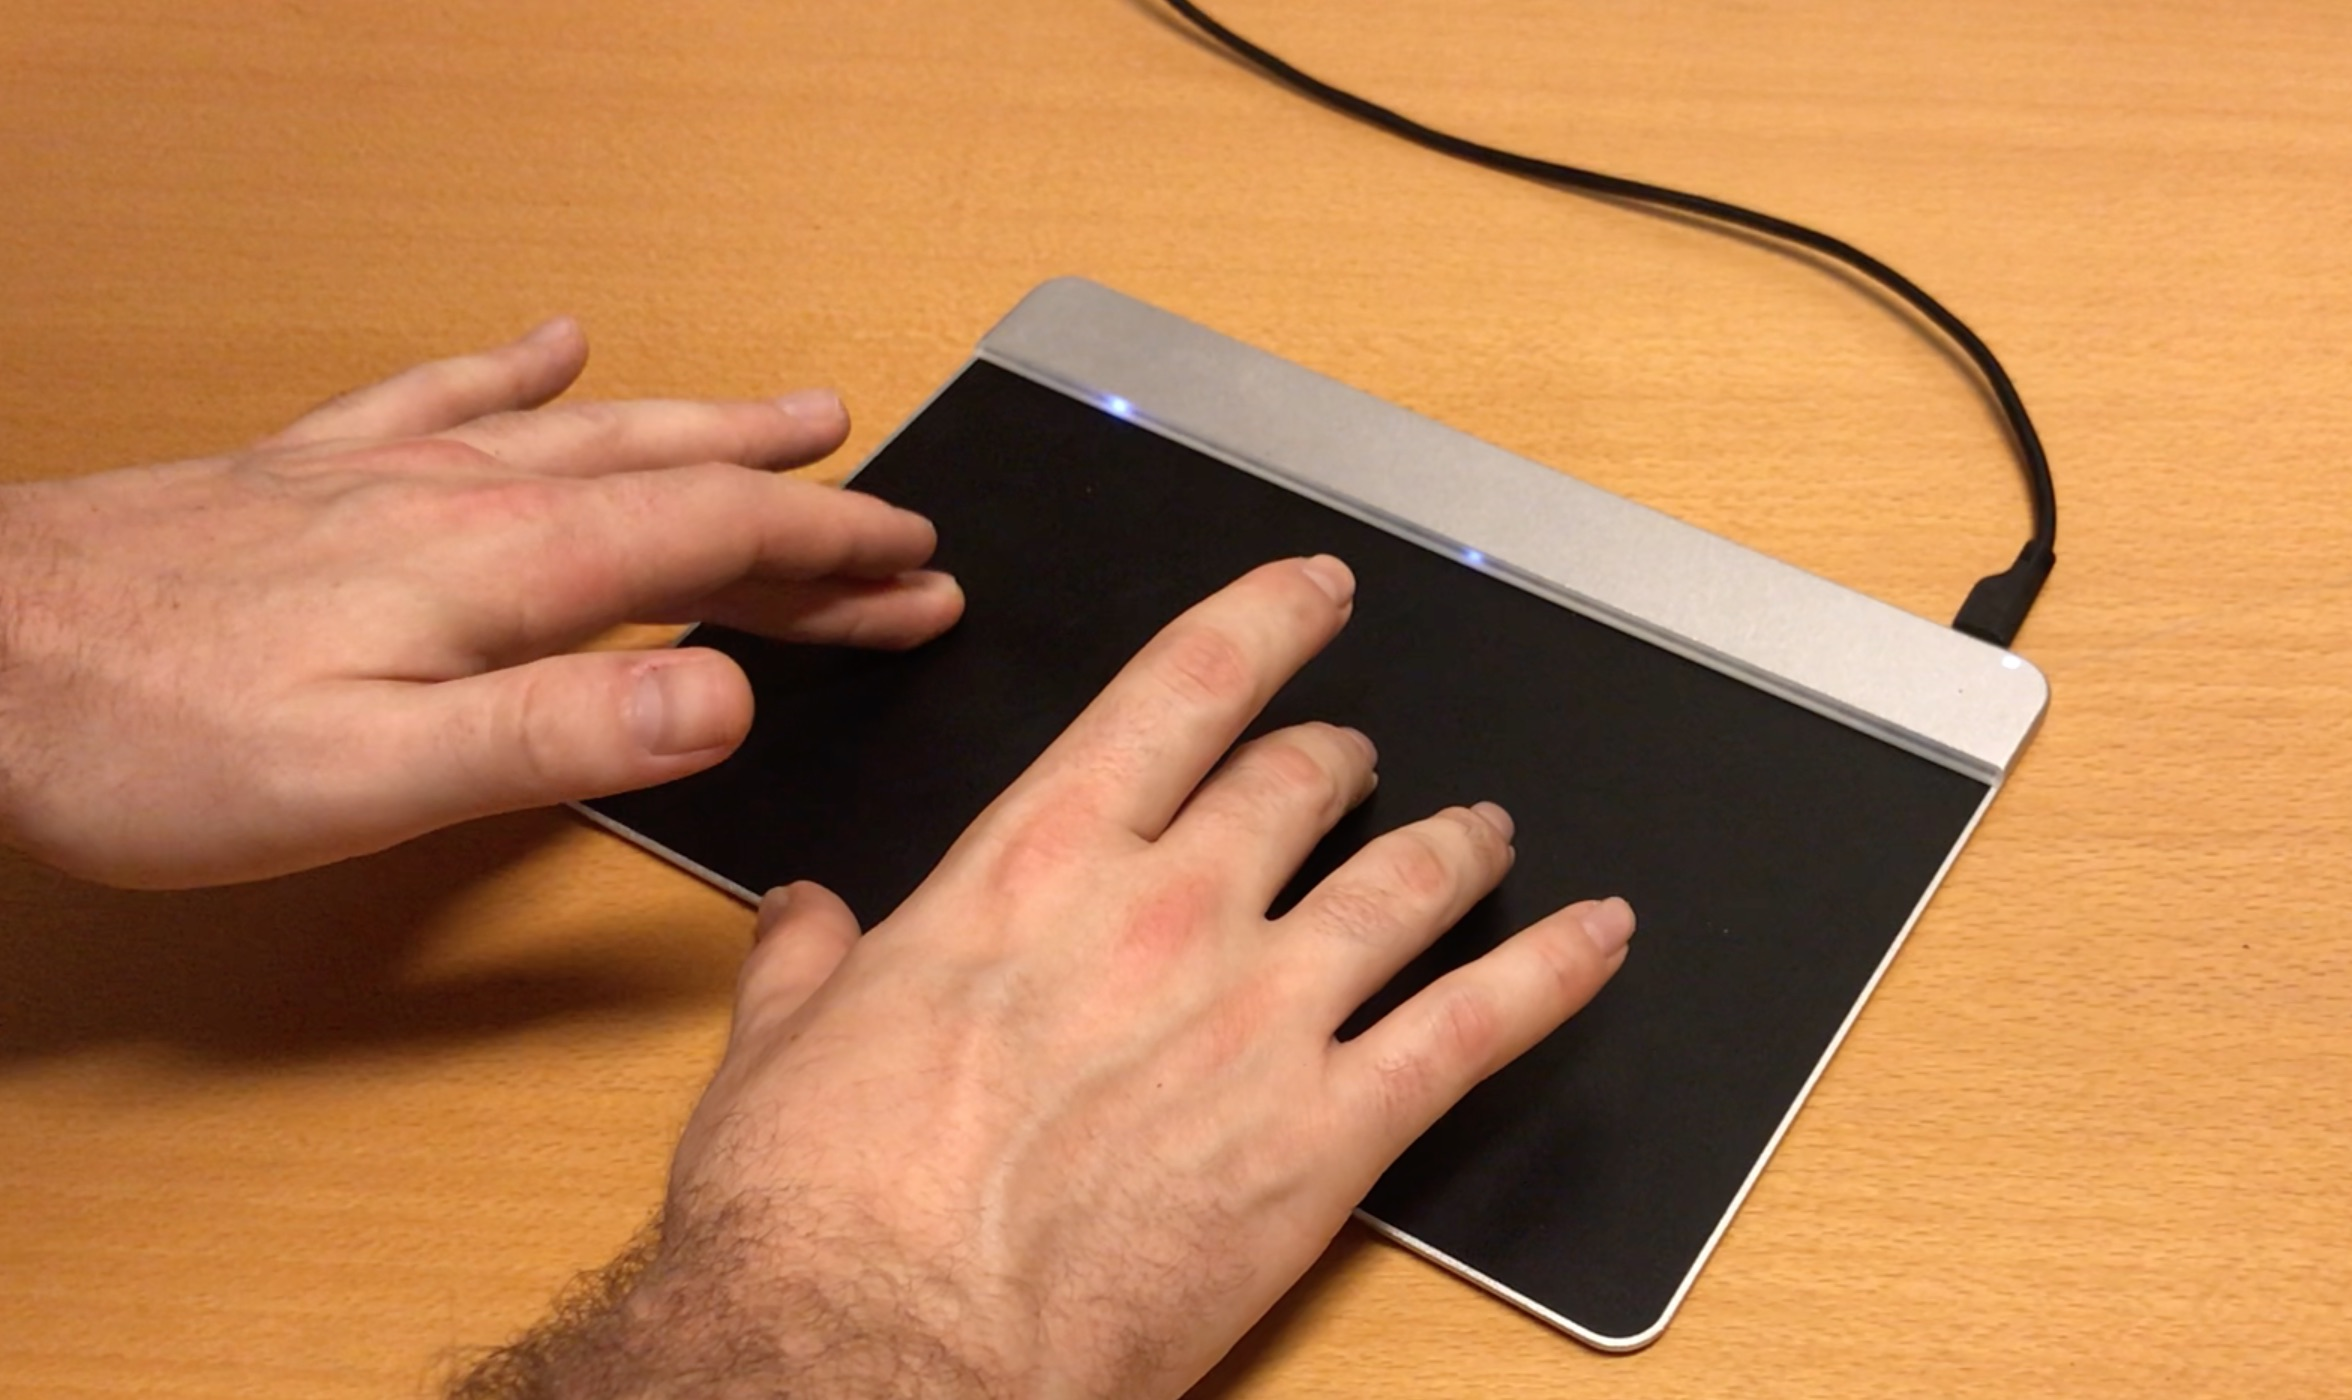
\includegraphics[width=0.8\textwidth]{figures/contributions/realtime/senselHands.jpg}
    \caption{The Sensel Morph. \label{fig:sensel}}
\end{figure}

% \begin{figure}[h]
%     \centering
%     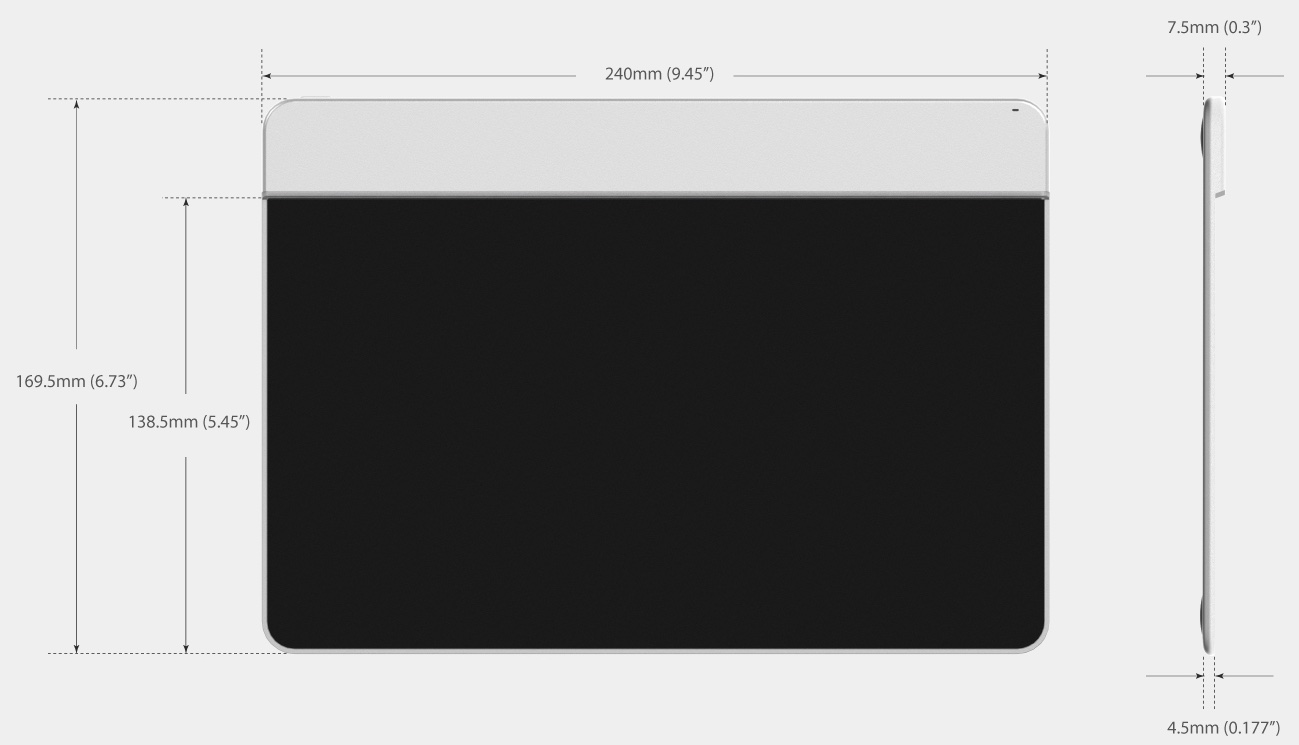
\includegraphics[width=\textwidth]{figures/realtime/dimensions.jpg}
%     \caption{Dimensions of the Sensel morph. (Taken from Sensel website with permission.) \label{fig:senselDims}}
% \end{figure}


\subsection{PHANTOM Omni}\label{sec:phantomOmni}
The PHANTOM Omni, or Omni for short, is a six-degrees-of-freedom device that provides force and vibrotactile feedback (see Figure \ref{fig:omni})

Other work using the Omni in a musical context, specifically for plucking a virtual guitar string, was done by Passalenti et al. in \cite{passalenti2019a, passalenti2019b} and Fontana et al. in \cite{Fontana2020}

\begin{figure}[h]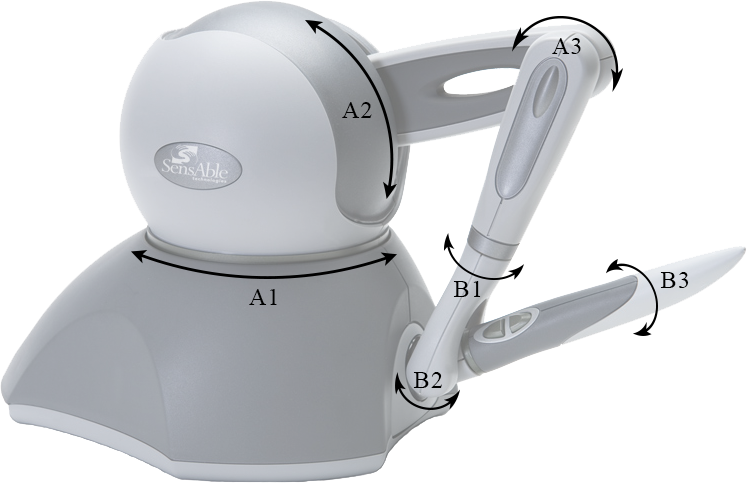
\includegraphics[width=0.8\textwidth]{figures/contributions/realtime/omniSchematic.png}
    \centering
      \caption{The PHANTOM Omni haptic device. The device has six axes of rotation (6-DoF), three of which provide force feedback (A1-3), and three that only track position (B1-3). \label{fig:omni}}
\end{figure}

\section{Discussion and Conclusion}
No proper comparisons have been done between MATLAB and C++

examples can be found in \cite{Webb2015} and \cite{Bilbao2019CMJb}





\subsection{Translating MATLAB to C++}
Indexing in
Matlab is 1-based, meaning that the index of a vector starts at 1. If \texttt{u} is a vector with 10 elements, the first element is retrieved as \texttt{u(1)} and the last as \texttt{u(10)}. C++, on the other hand, is 0-based and retrieving the first and last element of a size-10 vector happens through \texttt{u[0]} and \texttt{u[9]}respectively. 

\section{Considerations in real-time FD schemes}

Some of the things I learned (the hard way)...
\begin{itemize}
    \item Create a limiter
    \item Structure your application into classes 
    \item Use pointer switches
    \item Comment your code (hehe)
    \item Working with JUCE: select your audio output before building the application...
\end{itemize}

\subsubsection{Create a limiter}
Programming errors happen. To save your speakers, headphones or -- most importantly -- your ears, create a limiter. 

\setlstCpp
\begin{lstlisting}
double limit (double val)
{
    if (val < -1)
    {
        val = -1;
        return val;
    }
    else if (val > 1)
    {
        val = 1;
        return val;
    }
    return val;
}
\end{lstlisting}

\setlstMAT
\begin{lstlisting}
for  i = 0:lengthSound
    uNext = ...
end
\end{lstlisting}

\subsubsection{Denormalised numbers}
The damping present in FD schemes causes the state of the system to exponentially decay. What this means for the values of the state vectors in implementation, is that they keep getting closer to $0$ but never reach it. 

After a long period of time, which depends on the value of the damping coefficients, state values can get in the range of \textApprox$10^{-307}$! Numbers in this range are referred to as \textit{denormalised numbers} and operations with these are ``extremely slow'' \cite{CPPdenormalised}.

Although it rarely happens that numbers end up in this range, especially when the application is continuously interacted with, it is good to account for the possibility. For example, due to the very high damping of the body in the Tromba Marina application in Chapter \ref{ch:tromba}, denormalised numbers appear after \textApprox 10 s of not interacting with the instrument, and the CPU usage shoots up. There are specific processor flags that can be activated to truncate denormalised numbers to 0. To retain generality (cross-platform, various processors), one could implement a simple check per buffer to see whether values are smaller than e.g. $10^{-250}$ and truncate all values of that system to $0$. 


\section{Considerations for translating MATLAB to C++}
Although the \texttt{MATLAB} language, referred to throughout this thesis, is an excellent prototyping tool

This section will provide some considerations when moving from MATLAB to C++ 

It is usually a good idea to prototype a physical modelling application in \texttt{MATLAB} for various reasons, but  reasons: 1) Easier to debug, 2) Plotting functionality, 3) No need for memory handling, 4) no headphone blowup due to instability through programming errors



